\documentclass[a4paper,10pt, leqno]{article}
\usepackage[utf8]{inputenc}
\usepackage[bulgarian]{babel}
\newcommand{\HRule}{\rule{\linewidth}{0.5mm}}
\usepackage{amsmath}
\usepackage[unicode]{hyperref}
\hypersetup{
  colorlinks=true,
  linkcolor=black,
  pdftitle={Проект по ПФНРсСУБД2},
  pdfauthor={Валентина Динкова, Емил Станчев},
  pdfsubject={Бази от данни},
  pdfcreator={Емил Станчев, Валентина Динкова}
}
\usepackage{yfonts}
\usepackage{amsthm}
\usepackage {amssymb}
\usepackage{graphicx}
% for source code inclusion
\usepackage{listings}
\renewcommand{\lstlistingname}{\bfseries Файл}
\lstset{ language=Matlab, caption=\lstname, numbers=left, numberstyle=\tiny}
\lstset{keywordstyle=\bfseries}
\lstset{commentstyle=\color{darkgray}}
%\lstset{frame=T}
\newcommand{\attr}[1] {\texttt{#1}}
\newcommand{\enti}[1] {\textbf{#1}}
\newcommand{\re}[1] {\texttt{#1}}
\newcommand{\la}[1] {\textsl{#1}}
\newcommand{\rela}[1] {\textsl{#1}}
\newcommand{\func}[1] {\texttt{#1}}
\newcommand{\figref}[1] {Фигура \ref{#1}}

\begin{document}

% TITLE PAGE
\begin{titlepage}
  \begin{center}
    \textsc{СУ ``Св. Климент Охридски''\\
    Факултет по математика и информатика
    }\\[5cm]

    \textsc{\large Курсов проект по \\
	   	   Проектиране на физическо ниво и реализация със СУБД II
    }\\[0.5cm]
    \HRule \\[0.4cm]
    { \Large \bfseries База от данни за система за електронно обучение\\ \\[0.4cm]
    }\\[0.4cm]
    \HRule \\[6cm]
    \begin{minipage}{0.49\textwidth}
      \begin{flushleft} \large
	\emph{Автори:}\\
	Валентина Динкова,\\
	{\small ф.н.71112}\\
	Емил Станчев\\
	{\small ф.н.71100}\\
      \end{flushleft}
    \end{minipage}
    \begin{minipage}{0.49\textwidth}
      \begin{flushright} \large
	\emph{Ръководители:} \\
	доц. В. Димитров\\
	ас. Р. Горанова
      \end{flushright}
    \end{minipage}
    \vfill
    {\large \today}
  \end{center}
\end{titlepage}

\tableofcontents
\newpage

	\section{Описание}
	  Проектът представлява модел и примерна реализация на база от данни, предназначена за приложение за електронно обучение.
	  В него учителите качват материали за различни курсове, студентите обсъждат във форум различни теми, свързани с курсовете,
	  както и	административни въпроси. Учителите могат да качват задания с определен краен срок, за които студентите получават оценка.
	  Студентите могат да дават оценка на преподавателите в даден курс. Всички потребители се идентифицират с парола и email адрес.

	\section{Множества същности}
	Най-важните множества същности са:
	\begin{description}
	    \item[\enti{Course}]
	      Курс с име \attr{name} за дадена година. Може да има курсове с еднакви имена в различни години, затова ключът се състои
	      от името и годината на курса. Освен това има опционална парола \attr{password} за записване на курса. Пази се и броят на записаните
	      в курса студенти \attr{numEnrolled}. Всеки курс има един титуляр \attr{titular} и други учители \re{OtherTeachers}.
	      Всеки курс има категория \enti{Category}.
	      Всеки студент \enti{StudentProfile}, записан чрез \re{Enrolled} получава оценка за дадения курс \re{CourseGrade}, която има стойност
	      \attr{value}.
	    \item[\enti{User}]
	      Потребител, който има парола \attr{password}, \attr{email}, и имена \attr{first name}, \attr{last name}.
	      Всеки потребител има поне едно от \enti{StudentProfile} и \\
	      \enti{TeacherProfile}, които са слаби множества същности.
	    \item[\enti{Assignment}]
	      Задание, което има краен срок \attr{deadline}, максимален брой точки, които дава заданието \attr{max points}, заглавие \attr{title},
	      описание \attr{description}, уникален номер \attr{number} и дата на създаване \attr{created at}. Авторът на всеки \enti{Assignment}
	      е \enti{TeacherProfile} на някой \enti{User}. Всеки \enti{Assignment} може да има чрез \re{Attached} прикачени файлове \enti{File},
	      които имат име \attr{name}
	      и път \attr{path}, който е ключ за файла. Всяко задание принадлежи на даден курс.
	    \item[\enti{Resource}]
	      Ресурс, който принадлежи на даден \enti{Course}, напр. лекция, публикация и др. 
	      Ресурсът може да има прикачени файлове.
	    \item[\enti{ForumThread}]
	      Тема в дискусионния форум на даден курс, която има заглавие \attr{title} и тяло \attr{body}. Всяка тема може да има
	      отговори \enti{ForumReply}. Всички теми или отговори имат автори, които са \enti{User}.
	    \item[\enti{News}]
	      Новина относно курс \enti{Course}. Автори на новините са \enti{TeacherProfile}.
	    \item[\enti{Notification}]
	      Известие за настъпило събитие, като например прибавяне или изтриване на \enti{Assignment}, \enti{ForumReply} и др.
	\end{description}
      \section{ER Модел}
      Диаграмата на \la{Entity Relationship} модела е показана на \figref{fig:er}.
      \begin{figure}
	\label{fig:er}
      	\caption{\la{Entity Relatioinship} диаграма}
	 \centering
	 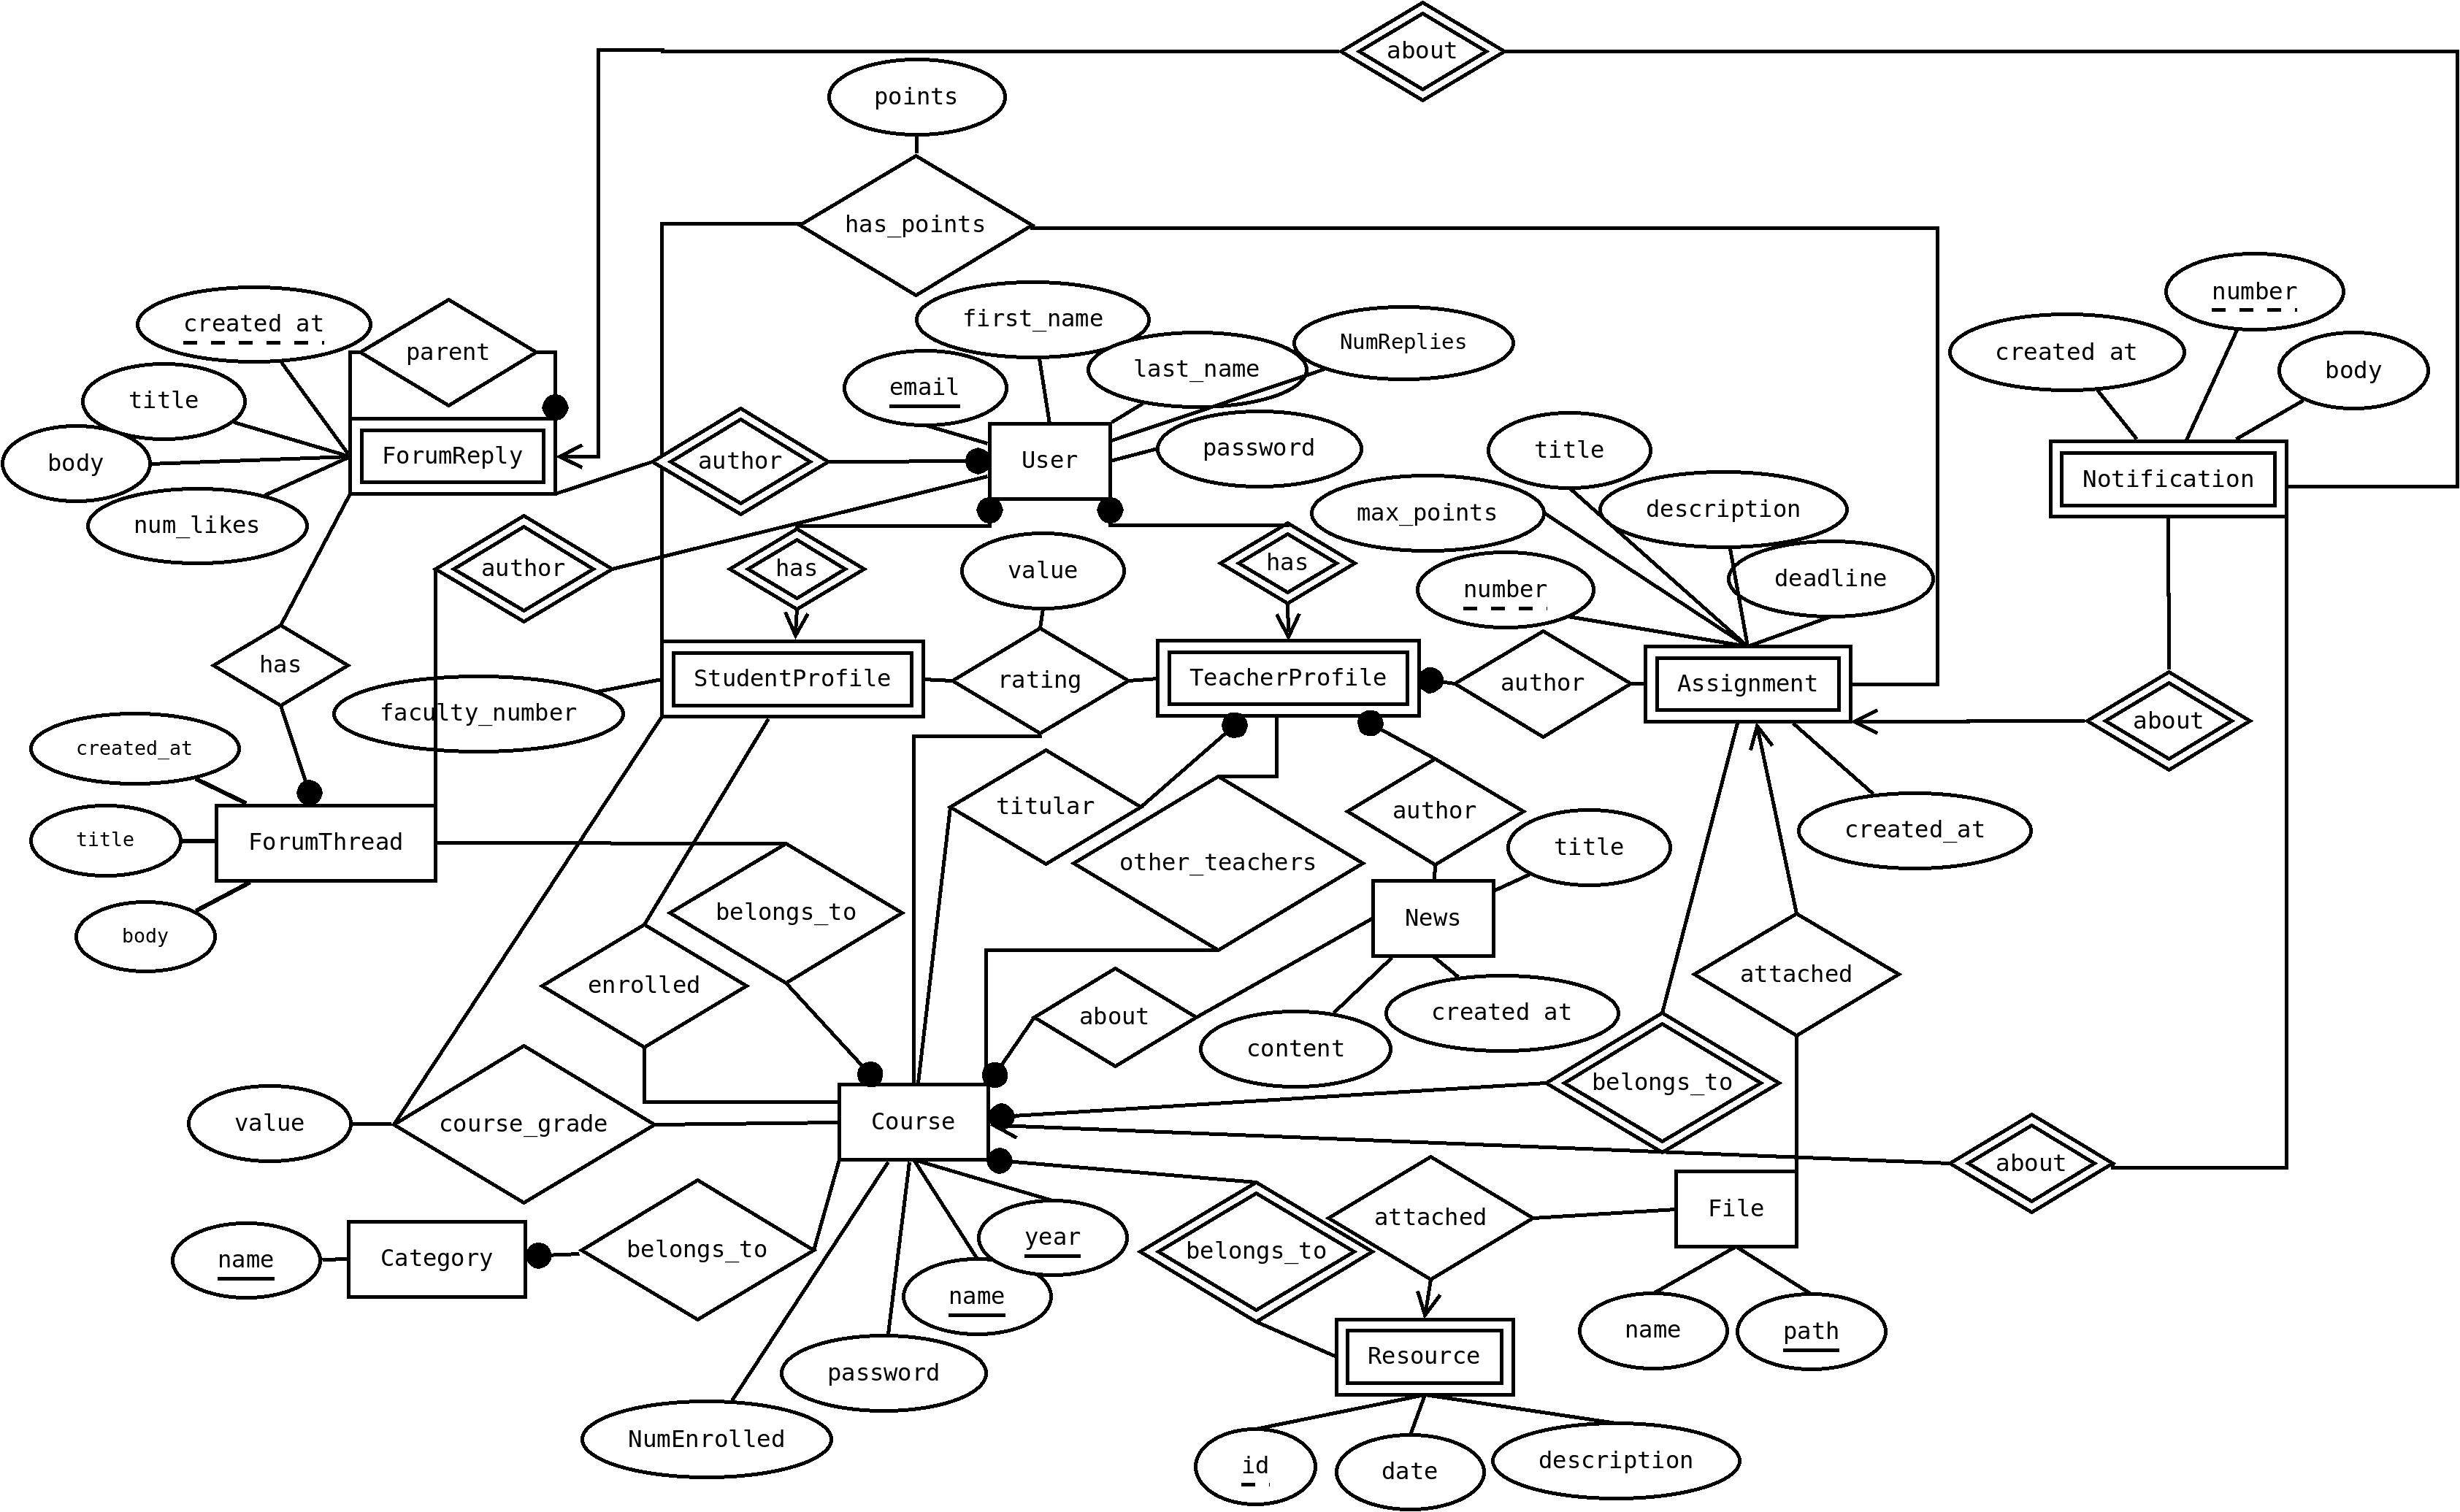
\includegraphics[width=21cm, angle=90]{../entity_relationship.jpeg}
      \end{figure}

      \section{Релационен модел}
      При преобразуването на \la{Entity Relationship} модела в релационен модел всички \la{много-към-едно} връзки са преобразувани
      в две релации вместо в три, като е използван \la{foreign key} в релацията за множеството, което стои от страната \la{много}.
      Множествата същности \enti{File} и \enti{Notification} са преобразувани в релации съответно \rela{AssignmentFile}, \rela{ResourceFile}
      и \rela{CourseNotificaiton}, \rela{AssignmentNotification} и \rela{ForumReplyNotification}. Това е направено, за да може да се
      създаде \la{foreign key} от страна на \enti{File} и \enti{Notification}.
      Всички ключове са преобразувани до \emph{минимални} такива.

      Диаграмата на релационния модел е показана на \figref{fig:rel}.
      \begin{figure}
	\label{fig:rel}
      	\caption{Релационен модел}
	 \centering
	 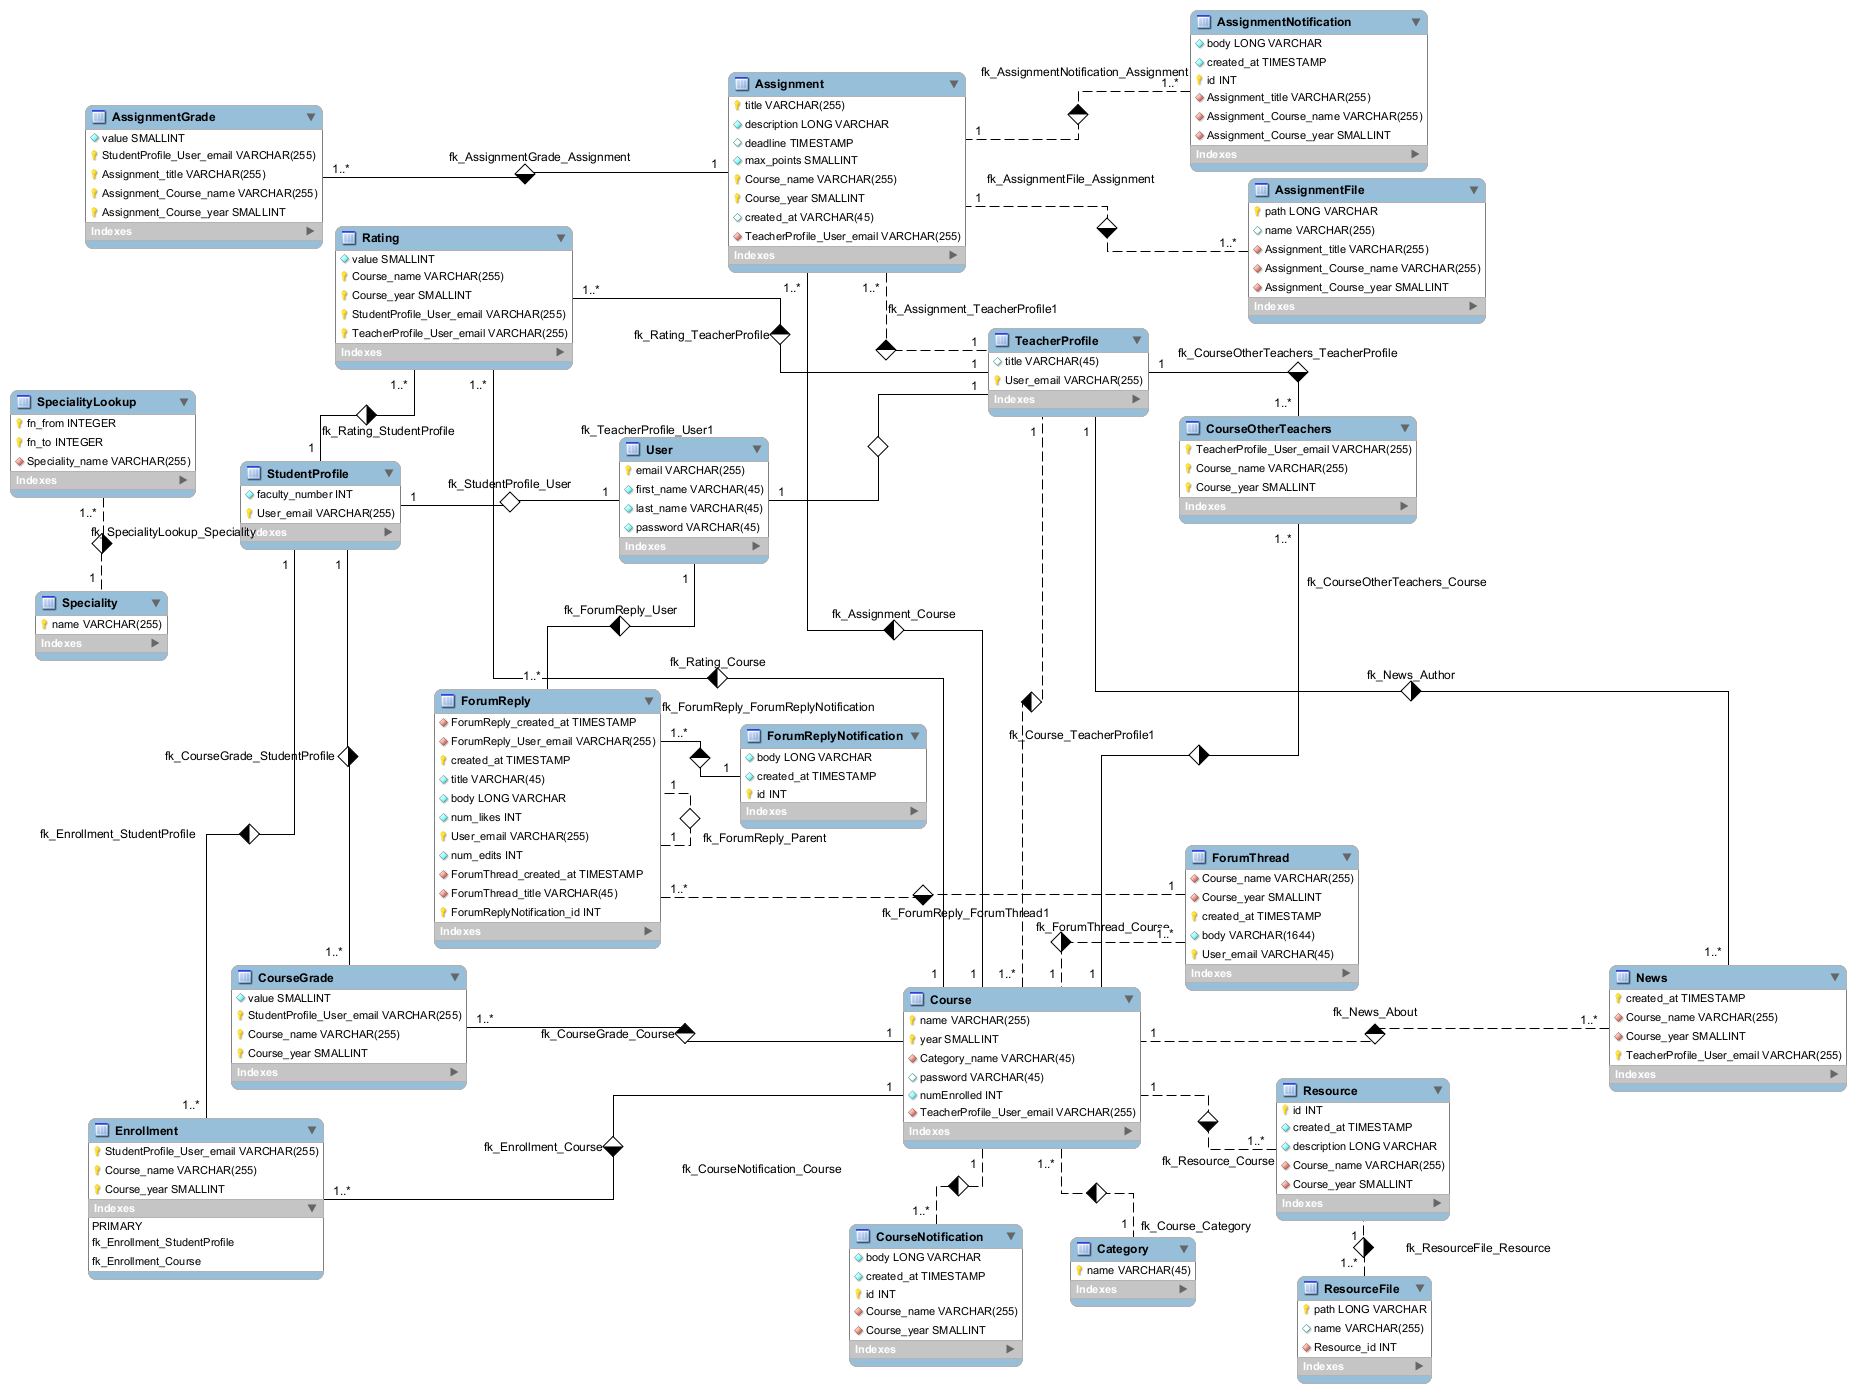
\includegraphics[width=21cm, angle=90]{../relational_model.png}
      \end{figure}

      \section{Ограничения}
      Всички подходящи \la{foreign key} ограничения са наложени. Всички атрибути като \attr{numEnrolled}, \attr{num\_likes} и т.н.
      са ограничени до неотрицателни стойности. Стойността на \attr{year} атрибута на \rel{Course} е ограничена до
      число между $1000$ и $9999$. За всеки \rel{ForumReply} е наложено ограничението той да е създаден по-късно от родителя си.
      Всички пароли се изисква да са с дължина най-малко $5$. За релацията \rel{SpecialityLookup} се проверява дали \attr{fn\_from} $\leq$ \attr{fn\_to}.


      \section{Функции}
       \begin{description}
	 \item[\func{get\_speciality(fn INT) RETURNS VARCHAR(255)}]
	   Връща името на специалността на даден студент (по факултетен номер \attr{fn}),
	   използвайки релацията \rel{SpecialityLookup}, в която са дефинирани интервали от факултетни номера
	   и съответстващи имена на специалности. 	 \item[ \func{count\_speciality\_students(spec VARCHAR(255)) RETURNS INT}]
	   Връща броя на студентите от дадена специалност.
	 \item[ \func{teacher\_mean\_rating(teacher\_email VARCHAR(255)) RETURNS DOUBLE}]
	   Връща средния рейтинг на даден учител - сумата от рейтингите от всички курсове, разделена на броя на всички рейтинги.
	 \item[ \func{all\_course\_teachers(n VARCHAR(255), y INT) RETURNS TABLE(User\_email VARCHAR(255))}]
	   Връща релация, включваща всички учители за даден курс - титуляра и другите учители, ако има такива.
	   \attr{n} и \attr{y} са името и годината на курса.
	 \item[ \func{too\_old(t TIMESTAMP) RETURNS INT} ]
	   Проверява дали времето \attr{t} не определя асоцииран с него запис кат ``прекалено стар'', т.е. по-стар от $5$ дни.  Връща $0$ или $1$.
       \end{description}

      \section{Тригери}
       \la{SQL} тригерите, дефинирани в проекта, са:
       \begin{description}
	 \item[\func{tr\_new\_reply\_notify AFTER INSERT ON ForumReply}]
	 \item[\func{tr\_new\_assignment\_notify AFTER INSERT ON Assignment}]
	 \item[\func{tr\_deleted\_assignment\_notify AFTER DELETE ON ForumReply}]
	 \item Тези тригери създават известия за съответните събития.
	 \item[\func{tr\_enrollment\_new\_count AFTER INSERT ON Enrollment}]
	 \item[\func{tr\_enrollment\_delete\_count AFTER DELETE ON Enrollment}]
	 \item Тези тригери увеличават или намаляват \attr{numEnrolled} на съответния курс,
	   когато в него се запише или отпише студент.

       \end{description}
      \section{Функции}
       \la{SQL} функциите, дефинирани в проекта, са:
       \begin{description}
	 \item[\func{get\_speciality(fn INT) RETURNS VARCHAR(255)}]
	   Връща името на специалността на даден студент (по факултетен номер \attr{fn}),
	   използвайки релацията \rel{SpecialityLookup}, в която са дефинирани интервали от факултетни номера
	   и съответстващи имена на специалности.
	 \item[ \func{count\_speciality\_students(spec VARCHAR(255)) RETURNS INT}]
	   Връща броя на студентите от дадена специалност.
	 \item[ \func{teacher\_mean\_rating(teacher\_email VARCHAR(255)) RETURNS DOUBLE}]
	   Връща средния рейтинг на даден учител - сумата от рейтингите от всички курсове, разделена на броя на всички рейтинги.
	 \item[ \func{all\_course\_teachers(n VARCHAR(255), y INT) RETURNS TABLE(User\_email VARCHAR(255))}]
	   Връща релация, включваща всички учители за даден курс - титуляра и другите учители, ако има такива.
	   \attr{n} и \attr{y} са името и годината на курса.
	 \item[ \func{too\_old(t TIMESTAMP) RETURNS INT} ]
	   Проверява дали времето \attr{t} не определя асоцииран с него запис кат ``прекалено стар'', т.е. по-стар от $5$ дни.  Връща $0$ или $1$.
       \end{description}

      \section{Процедури}
       \la{SQL} процедурите, дефинирани в проекта, са:
       \begin{description}
	 \item[\func{cleanup\_old\_notifications}]
	   Изтрива всички ``твърде стари'' известия според функцията \func{too\_old}.
	\item[\func{urgent\_assignment\_notifications}]
	   Проверява за задания, за които остава по-малко от $1$ ден до крайния срок и създава известия за тях.
       \end{description}
\end{document}
